\section{Introduction}

\margininfonote{Because the SDK is Eclipse-based, any features and customizations available to common Eclipse distributions can be used in the IDE. Additionally, resources and knowledge bases for Eclipse can be leveraged for information on navigation and settings of the IDE.}

This guide assumes that you have already installed the Xilinx SDK which can be done by following the snickerdoodle "Development Environment Setup" guide. This guide uses the Xilinx SDK 2015.2 installed on Windows 10. \\


\noindent
The SDK has an extensive built-in user guide which provides assistance on many common tasks such as creating and building projects and using the system debugger. The user guide can be found by navigating to \textit{\bfseries Help $\rightarrow$ Help Contents} from the menubar. This will launch the user guide in a web browser for navigation.


\section{Launching the SDK}
If the parent directory for the SDK has been added to the \Verb|$PATH| variable, then the SDK can be run by exectuting the \texttt{xsdk} command from a terminal: \\

\begin{lstlisting}
user@ubuntu:~$ xsdk
\end{lstlisting}

~\\
\noindent
After starting the SDK environment, you will be prompted to select a workspace in which to store application projects and files. This dialog can be bypassed in the future by selecting the "Use this as the default..." checkbox. \\

\begin{figure}[h]
	\centering
	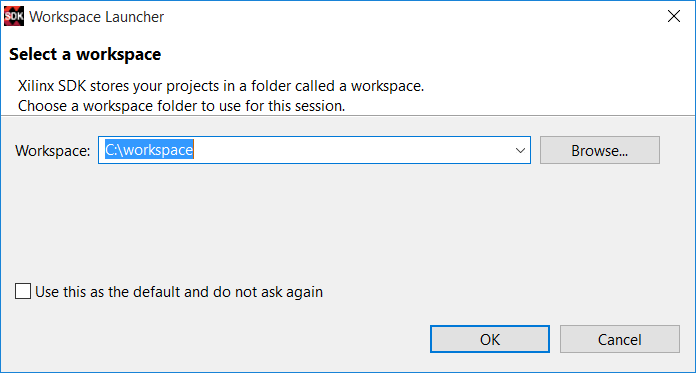
\includegraphics{images/Workspace_Selection.png}
	\caption{Selecting an SDK Workspace Path from the Workspace Launcher Dialog}
	\label{fig:workspacedialog}
\end{figure}


\section{Creating a Project}

\noindent
After selecting a workspace, the SDK environment will open and you will be able to create new projects. To create a new Linux project, start by navigating to \textit{\bfseries File $\rightarrow$ New $\rightarrow$ Application Project} from the menubar or \textit{\bfseries New $\rightarrow$ Application Project} from the toolbar as shown in \figref{fig:newproject}. \\

\begin{marginfigure}
	\centering
	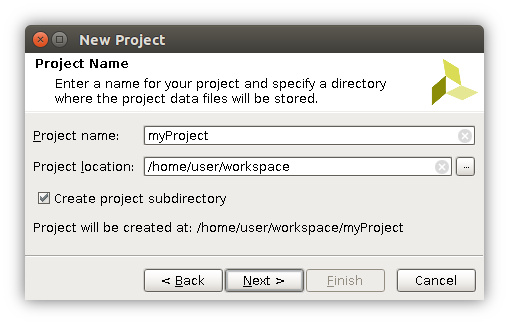
\includegraphics{images/New_Project.png}
	\caption[Starting a New Project from the Toolbar]{Starting a New Project from the Toolbar}
	\label{fig:newproject}
\end{marginfigure}


\noindent
From the "New Project" dialog, a project type can be selected. This will open the wizard for the selected project type, in this case an \textit{Application Project}. "Application Project" can be selected from the "Xilinx" folder. This will create a pre-configured project, ready to be cross-compiled using the Xilinx compiler toolchain and managed by the SDK. \\


\noindent
From within the \textit{Application Project Wizard}, the project can be named and a project type selected. For a Linux application, the OS Platform should be changed to "linux." The "Linux System Root" and "Linux Toolchain" do not need to be changed to build Linux applications for snickerdoodle. \\

\begin{figure}[h!]
	\centering
	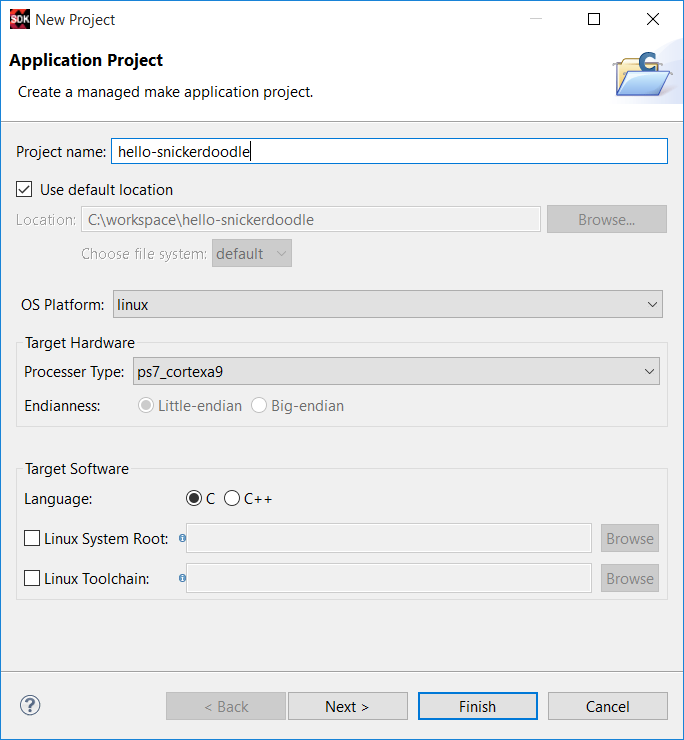
\includegraphics{images/New_Linux_Project.png}
	\caption{Creating a Linux Application in the Application Project Wizard}
\end{figure}

\noindent
To target a Linux system booting on the Cortex-A9 processor, select \texttt{ps7\_cortexa9} from the \textit{Processor Type} drop-down menu. Other options include \texttt{microblaze} for systems running on microblaze processors that have been synthesized in programmable logic. \\


\begin{figure}[h!]
	\centering
	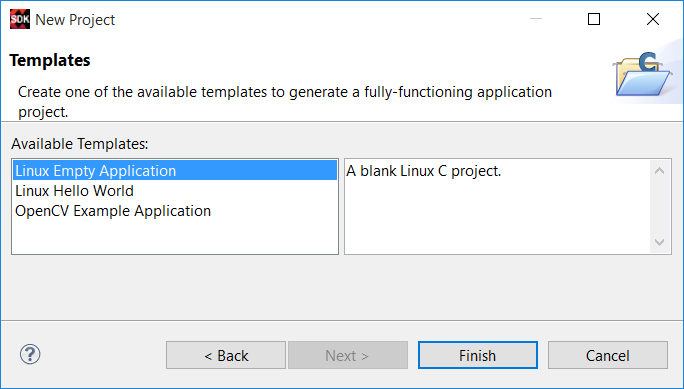
\includegraphics{images/Linux_Empty_Application.png}
	\caption{Finishing Application Project Generation by Selecting a Project Template}
\end{figure}

\noindent
After selecting \textit{\bfseries Next} from the \textit{Application Project Wizard}, a template for the application can be selected. For this example, the application project will be left empty by selecting the "Linux Empty Application" template. This will create a C project without any source files. \\



\noindent
Clicking \textit{\bfseries Finish} will generate the application project and make it available in the SDK environment's project explorer. 


\section{Create Project Source Files}


\begin{marginfigure}
	\centering
	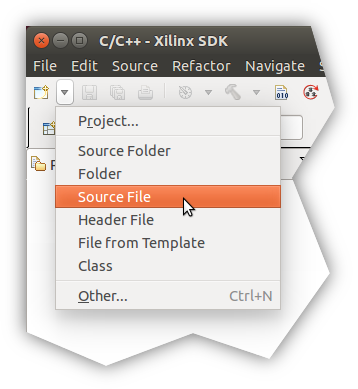
\includegraphics{images/New_File.png}
	\caption[Creating a New Source File from the Toolbar]{Creating a New Source File from the Toolbar}
	\label{fig:newfiletoolbar}
\end{marginfigure}


After the project is created, it can be populated with project files. The simplest case is a single file program. In this example, a single file named \texttt{main.c} is created and populated with the program's entry point function, \Verb|main()|. \\


\noindent
Creation of new files can be done by right-clicking on the desired parent directory or selecting \textit{\bfseries File} from the menubar, and selecting \textit{\bfseries New $\rightarrow$ Source File}. Source files can also be created, as shown in \figref{fig:newfiletoolbar}, by selecting \textit{\bfseries New $\rightarrow$ Source File} from the toolbar. \\

\begin{fullwidth}
\infonote{Additional information on configuring and customizing code templates can be found at \url{http://help.eclipse.org/mars/index.jsp?topic=\%2Forg.eclipse.cdt.doc.user\%2Freference\%2Fcdt_u_c_code_templates_pref.htm}}
\end{fullwidth}

\noindent
From the \textit{\bfseries New File} dialog, the file name (including extension), parent directory and source file template can be selected. Templates can be configured and customized to include common file elements such as headers and comments. \\

\begin{figure}[h!]
	\centering
	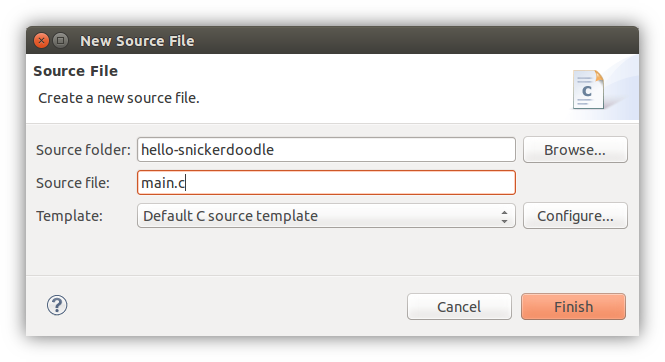
\includegraphics{images/New_Main.png}
	\caption{Selecting the File Name and File Template}
\end{figure}

\subsection{Writing Source Files}
The structure of applications for snickerdoodle takes the familiar form of any C/C++ Linux application. Project management and file structure will be recognizable to any user with some experience with C/C++ programming in an Eclipse environment. For this example, a simple "hello world" style program is generated by populating the \texttt{main.c} file with the following code: \\

\begin{lstlisting}[language=c]
/*
 *   File:    main.c
 */

#include <stdio.h>
#include <stdlib.h>

int main( int argc, char * argv[] )
{
    printf( "Hello snickerdoodle!\n" );

    return EXIT_SUCCESS;
}
\end{lstlisting}



\section{Building the Application}

Cleaning and building the application can be done by selecting \textit{\bfseries Project $\rightarrow$ Clean..} which will  as shown in \figref{fig:cleanbuild}. \\

\begin{figure}[h]
	\centering
	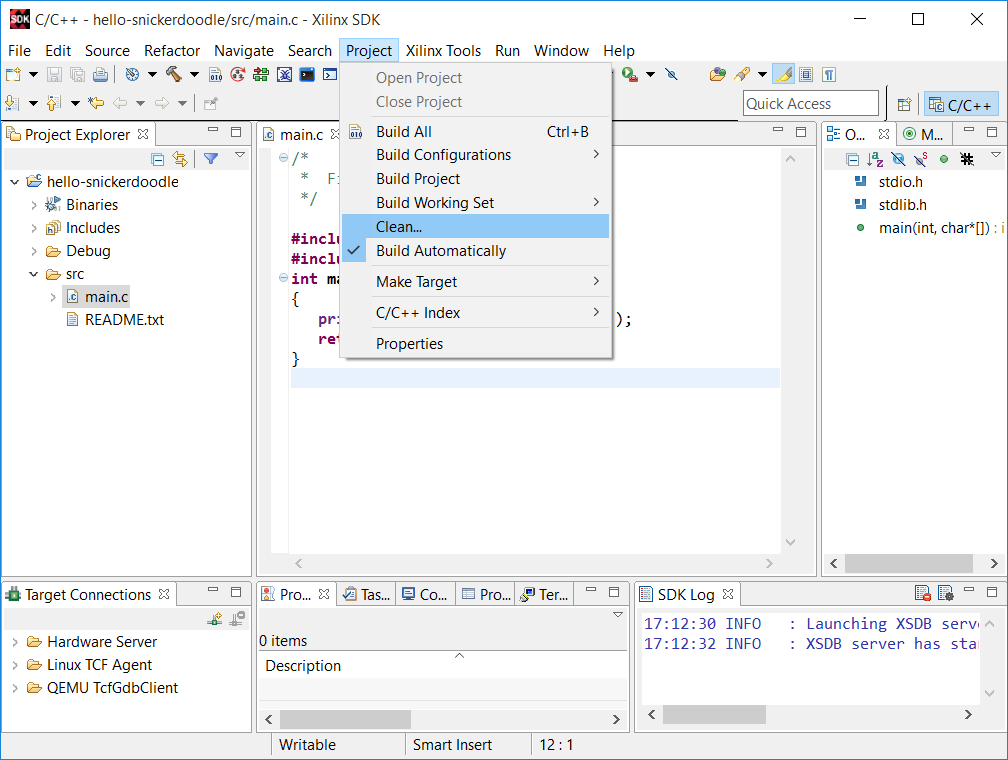
\includegraphics{images/Clean_Project.png}
	\caption{Clean and Build the Project from the Menubar}
	\label{fig:cleanbuild}
\end{figure}


\noindent
The invocation of the compiler toolchain can be seen in the console of the IDE. After a successful build, the console should show messages similar to the following: 

\begin{fullwidth}
\begin{lstlisting}[style=text,backgroundcolor=\color{white}]
17:33:01 **** Build of configuration Debug for project hello-snickerdoodle ****
make all 
'Building file: ../src/main.c'
'Invoking: ARM Linux gcc compiler'
arm-xilinx-linux-gnueabi-gcc -Wall -O0 -g3 -c -fmessage-length=0 -MT"src/main.o" -MMD -MP -MF"src/main.d" -MT"src/main.d" -o "src/main.o" "../src/main.c"
'Finished building: ../src/main.c'
' '
'Building target: hello-snickerdoodle.elf'
'Invoking: ARM Linux gcc linker'
arm-xilinx-linux-gnueabi-gcc  -o "hello-snickerdoodle.elf"  ./src/main.o   
'Finished building target: hello-snickerdoodle.elf'
' '
'Invoking: ARM Linux Print Size'
arm-xilinx-linux-gnueabi-size hello-snickerdoodle.elf  |tee "hello-snickerdoodle.elf.size"
   text	   data	    bss	    dec	    hex	filename
   1254	    292	      4	   1550	    60e	hello-snickerdoodle.elf
'Finished building: hello-snickerdoodle.elf.size'
' '

17:33:02 Build Finished (took 605ms)
\end{lstlisting}
\end{fullwidth}

\noindent
At this point, the Linux application has been compiled and the executable can be copied to \textit{ROOTFS}. The SD card can now be ejected and mounted on snickerdoodle where the system will be booted. The application can be executed from the command line of your booted snickerdoodle. Execution of the program should look like the following:

\begin{lstlisting}[%
  backgroundcolor=\color{black},
  basicstyle={\small\ttfamily\color{green}}
  ]
user@snickerdoodle~$ hello-snickerdoodle
Hello snickerdoodle!
\end{lstlisting}


